\chapter{Experimentación y resultados}\label{chapter:experimentation}

En este capítulo se procede al cumplimiento de los objetivos principales de este trabajo. Se mostrará cómo crear y configurar un cliente en Keycloak y por último, se procede a experimentación del sistema creado a través de un cliente realizado en \textit{Python}.

\section{Configuración de cliente Keycloak} \label{config-client}
 
%Para la ejecución de Keycloak se debe ejecutar el siguiente comando:
%
%\lstset{language=csh}
%\lstset{frame=lines}
%\lstset{caption={Ejecución de Keycloak}}
%\lstset{label={lst:runkecloak}}
%\lstset{basicstyle=\footnotesize}
%\begin{lstlisting}
%$ kc.sh start-dev
%\end{lstlisting}
%
%Por defecto \href{http://localhost:8080/}{\textcolor{blue}{http://localhost:8080/}}

Para la siguiente experimentación se ha utilizado una base de datos del Nodo Central a la cual se accede de forma remota a través de una VPN y accediendo a una IP. La máquina en la cual se hospeda tiene 1 GB de RAM. La computadora en la que se experimentó tiene  8 GB de RAM y 2.7 GHz Dual-Core Intel Core i5 de CPU.

 Luego de configurado LDAP y sincronizados los usuarios, Keycloak permite añadir clientes de forma sencilla. En las siguientes imágenes se muestra paso a paso como se agrega un nuevo cliente al sistema:

\begin{figure}[H]
	\centering
	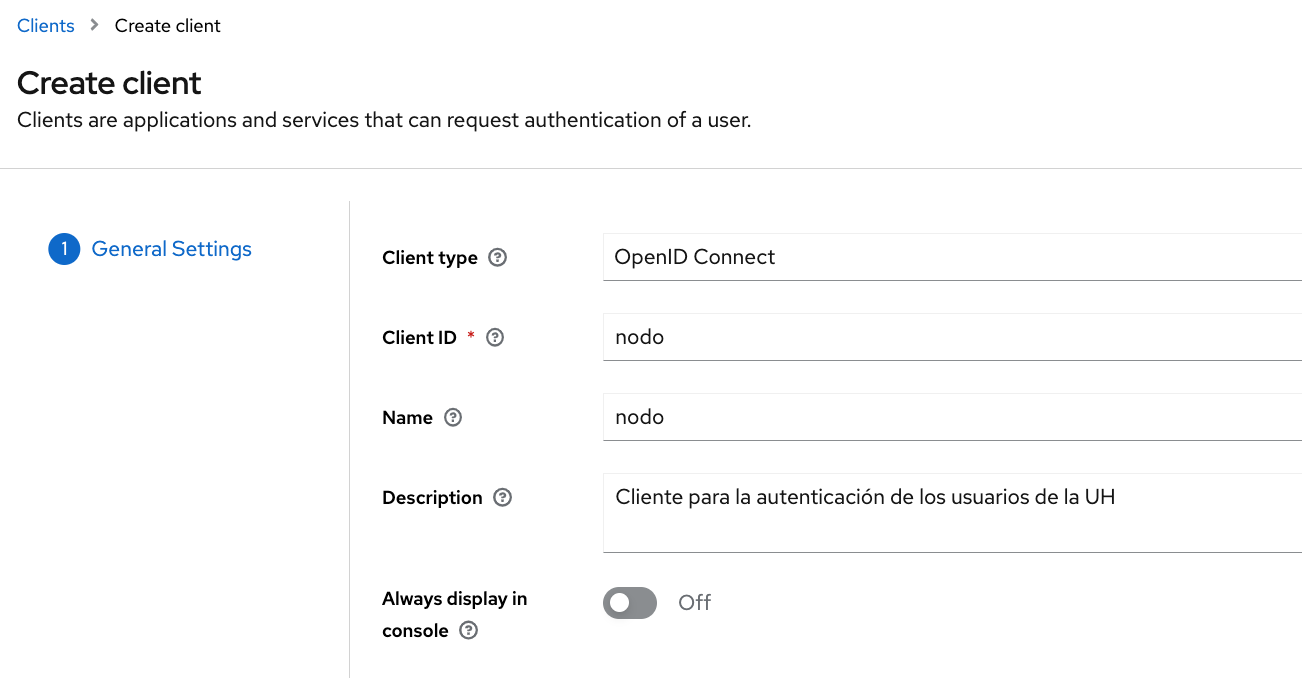
\includegraphics[width=1\linewidth]{Graphics/client_new1}
	\caption{Nuevo cliente en Keycloak}
	\label{fig:clientnew1}
\end{figure}

\begin{figure}[H]
	\centering
	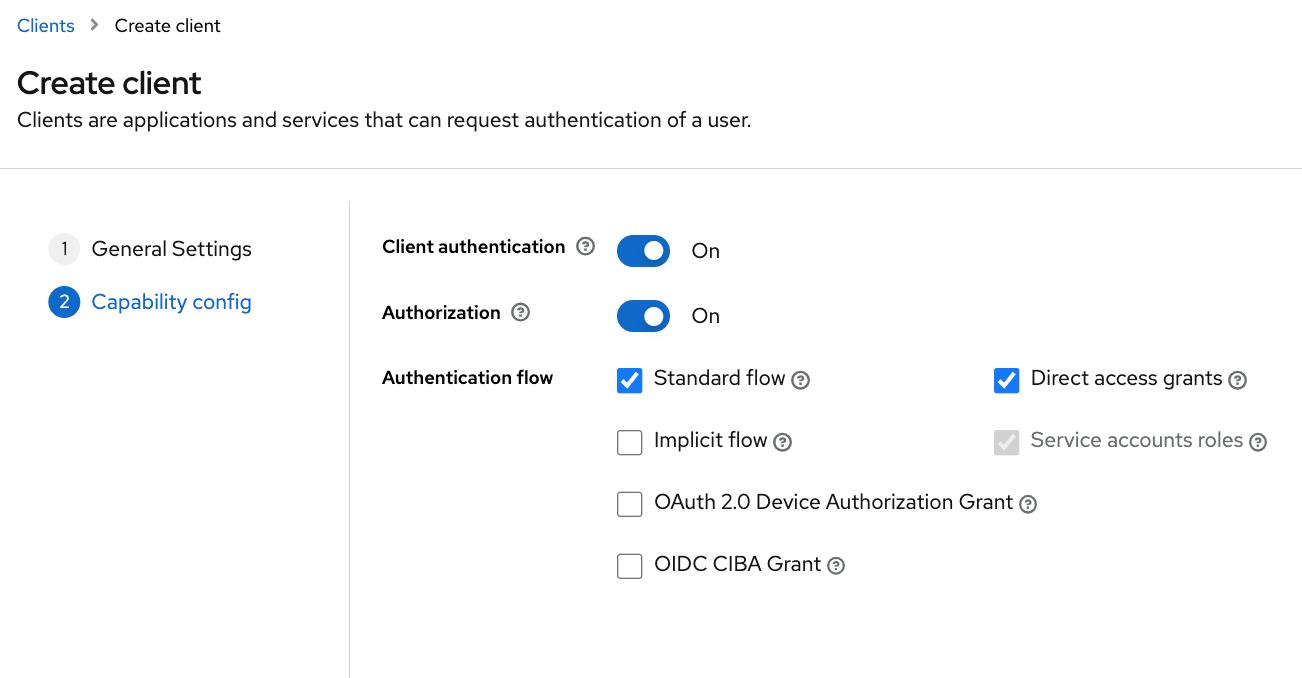
\includegraphics[width=1\linewidth]{Graphics/client_new2}
	\caption{Nuevo cliente en Keycloak}
	\label{fig:clientnew2}
\end{figure}

Luego se puede ver el nuevo cliente nodo en la lista de clientes:

\begin{figure}[H]
	\centering
	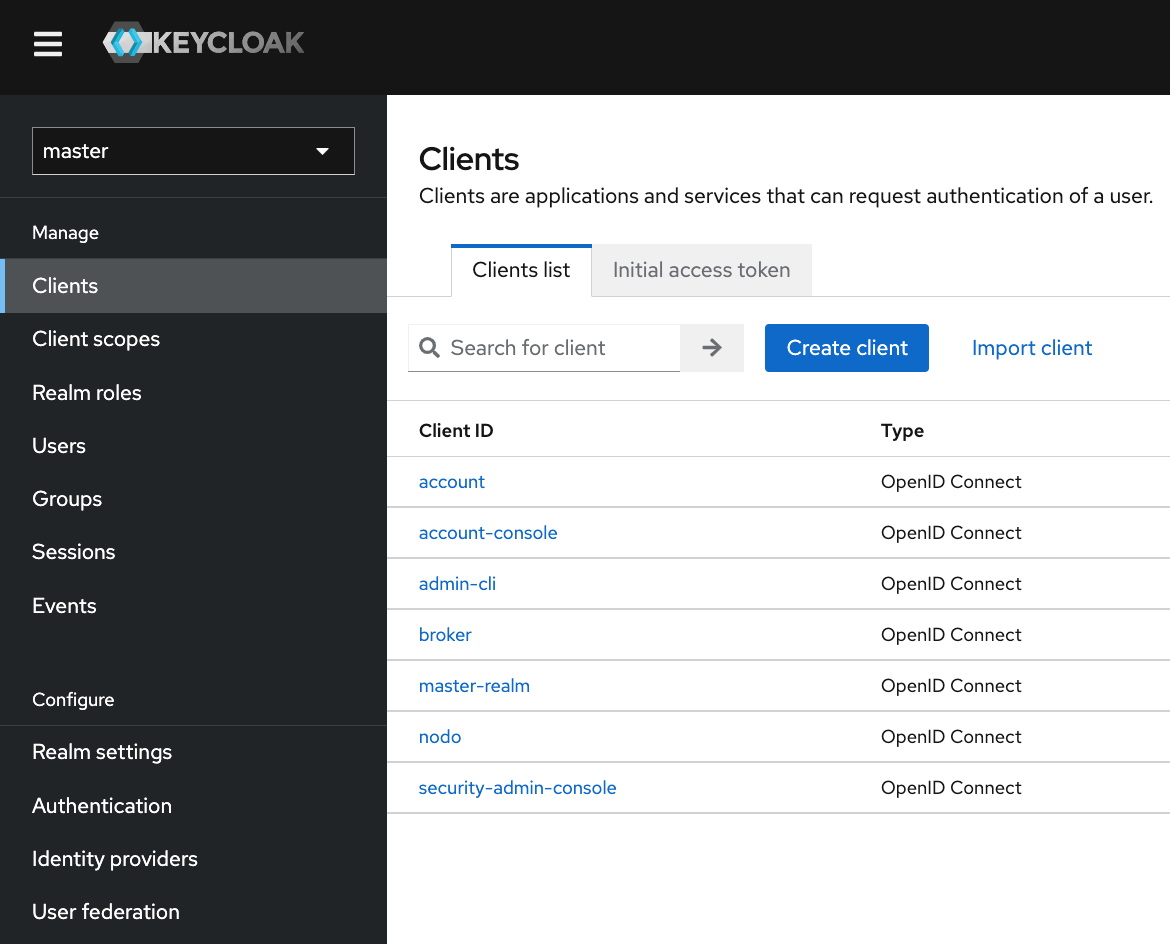
\includegraphics[width=0.9\linewidth]{Graphics/client_list}
	\caption{Lista de clientes}
	\label{fig:clientlist}
\end{figure}

Luego de crear el cliente, se puede este conectar a los servicios de Keycloak con la correcta configuración. Para ello será necesario utilizar las credenciales del cliente:

\begin{figure}[H]
	\centering
	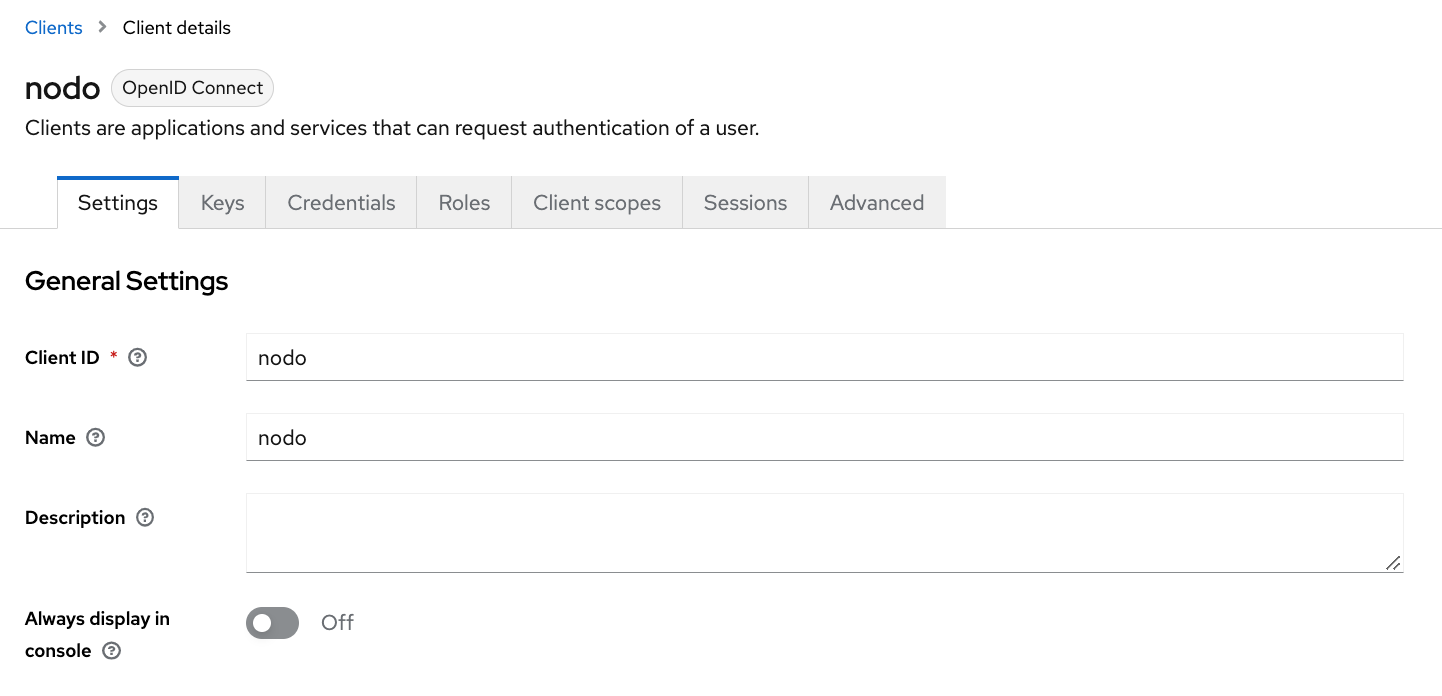
\includegraphics[width=0.9\linewidth]{Graphics/client_nodo}
	\caption{Cliente nodo}
	\label{fig:clientnodo}
\end{figure}

\begin{figure}[H]
	\centering
	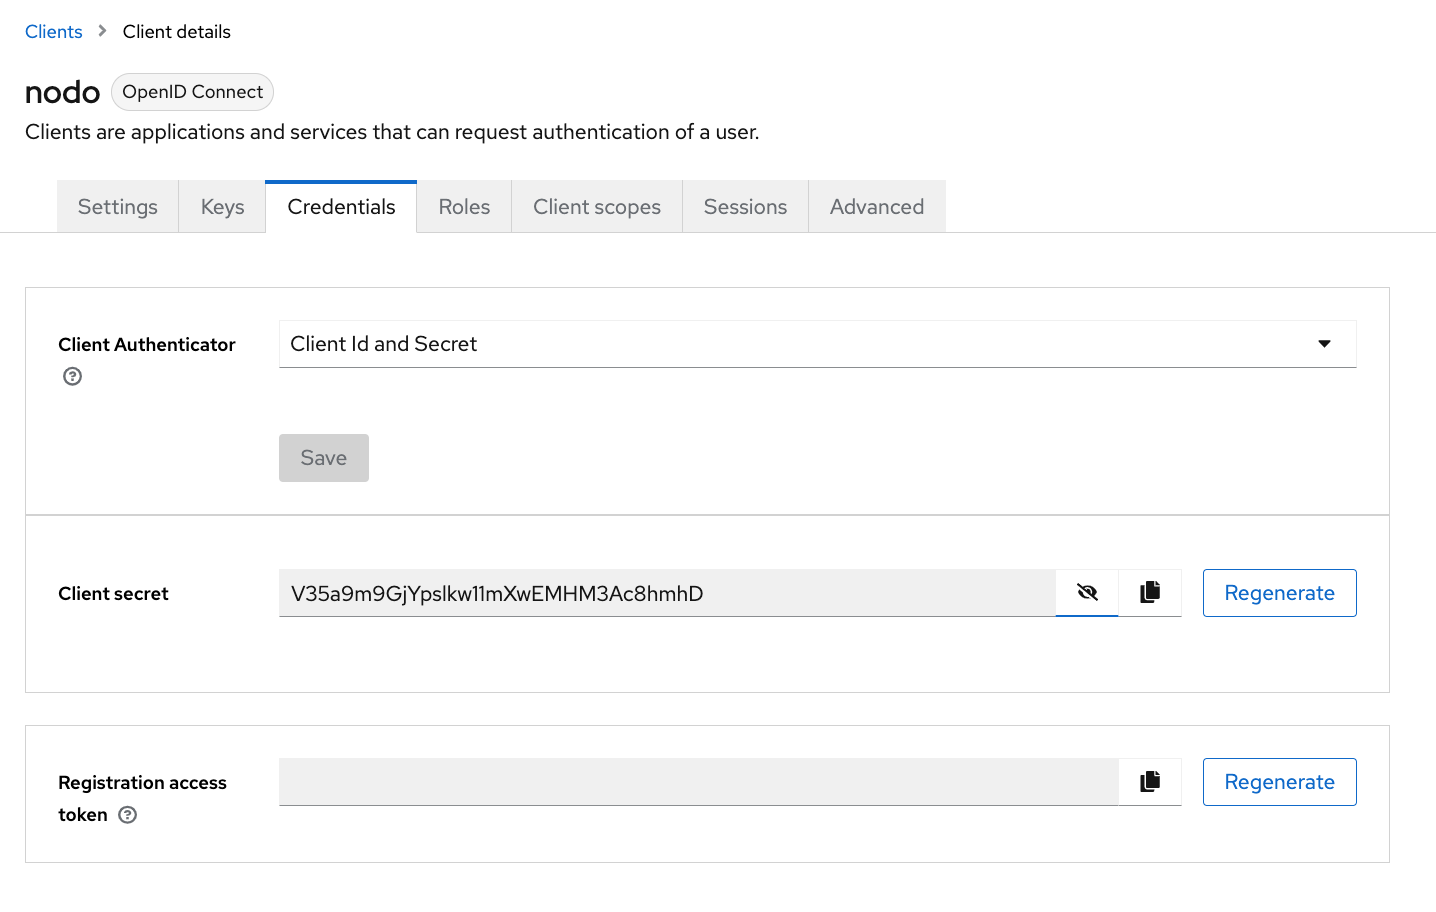
\includegraphics[width=0.9\linewidth]{Graphics/client_nodo_credentials}
	\caption{Credenciales del cliente nodo}
	\label{fig:clientnodocredentials}
\end{figure}

%\textcolor{red} {cómo se configura un cliente en keycloak?
%Qué endpoints expone la API de keycloak?
%Hablar sobre la biblioteca de python
%Poner el ejemplo de cómo se autentica}

\section{Creación de cliente Keycloak para obtención de token}

En el siguiente código se muestra cómo se puede conectar el cliente a Keycloak a través de la biblioteca \textbf{python-keycloak}. También se crea una interfaz básica con Flask para visualizar los resultados.


\lstset{language=Python}
\lstset{frame=lines}
\lstset{caption={Conexión de cliente a Keycloak}}
\lstset{label={lst:code_direct}}
\lstset{basicstyle=\footnotesize}
\begin{lstlisting}
from flask import Flask
from flask import Flask, render_template, request
from keycloak.keycloak_openid import KeycloakOpenID
from keycloak.exceptions import KeycloakAuthenticationError, KeycloakGetError

import json

app = Flask(__name__)

keycloak_open_id = KeycloakOpenID(server_url="http://localhost:8080/", 
	client_id="nodo", 
	realm_name="master", 
	client_secret_key="secret key")
keycloak_open_id.well_know()

@app.route('/login', methods=['POST', 'GET'])
def login():
	error = None
	if request.method == 'POST':
		username = request.form['username']
		success, result = valid_login(username, request.form['password'])
		if success:
			return log_the_user_in(username, result["access_token"], result["refresh_token"])
		else:
			error = result["error_description"]
	# The code below is executed if the request method
	# was GET or the credentials were invalid
	return render_template('login.html', error=error)

def valid_login(username, password):
	# import pdb
	# pdb.set_trace()
	try:
		token = keycloak_open_id.token(username, password)
	except (KeycloakAuthenticationError, KeycloakGetError) as e:
		return False, json.loads(e.error_message)
	return True, token

def log_the_user_in(username, token, refresh_token):
	return render_template('success.html', username=username, token=token, refresh_token=refresh_token)
\end{lstlisting}


El código anterior genera la siguiente interfaz:

\begin{figure}[H]
	\centering
	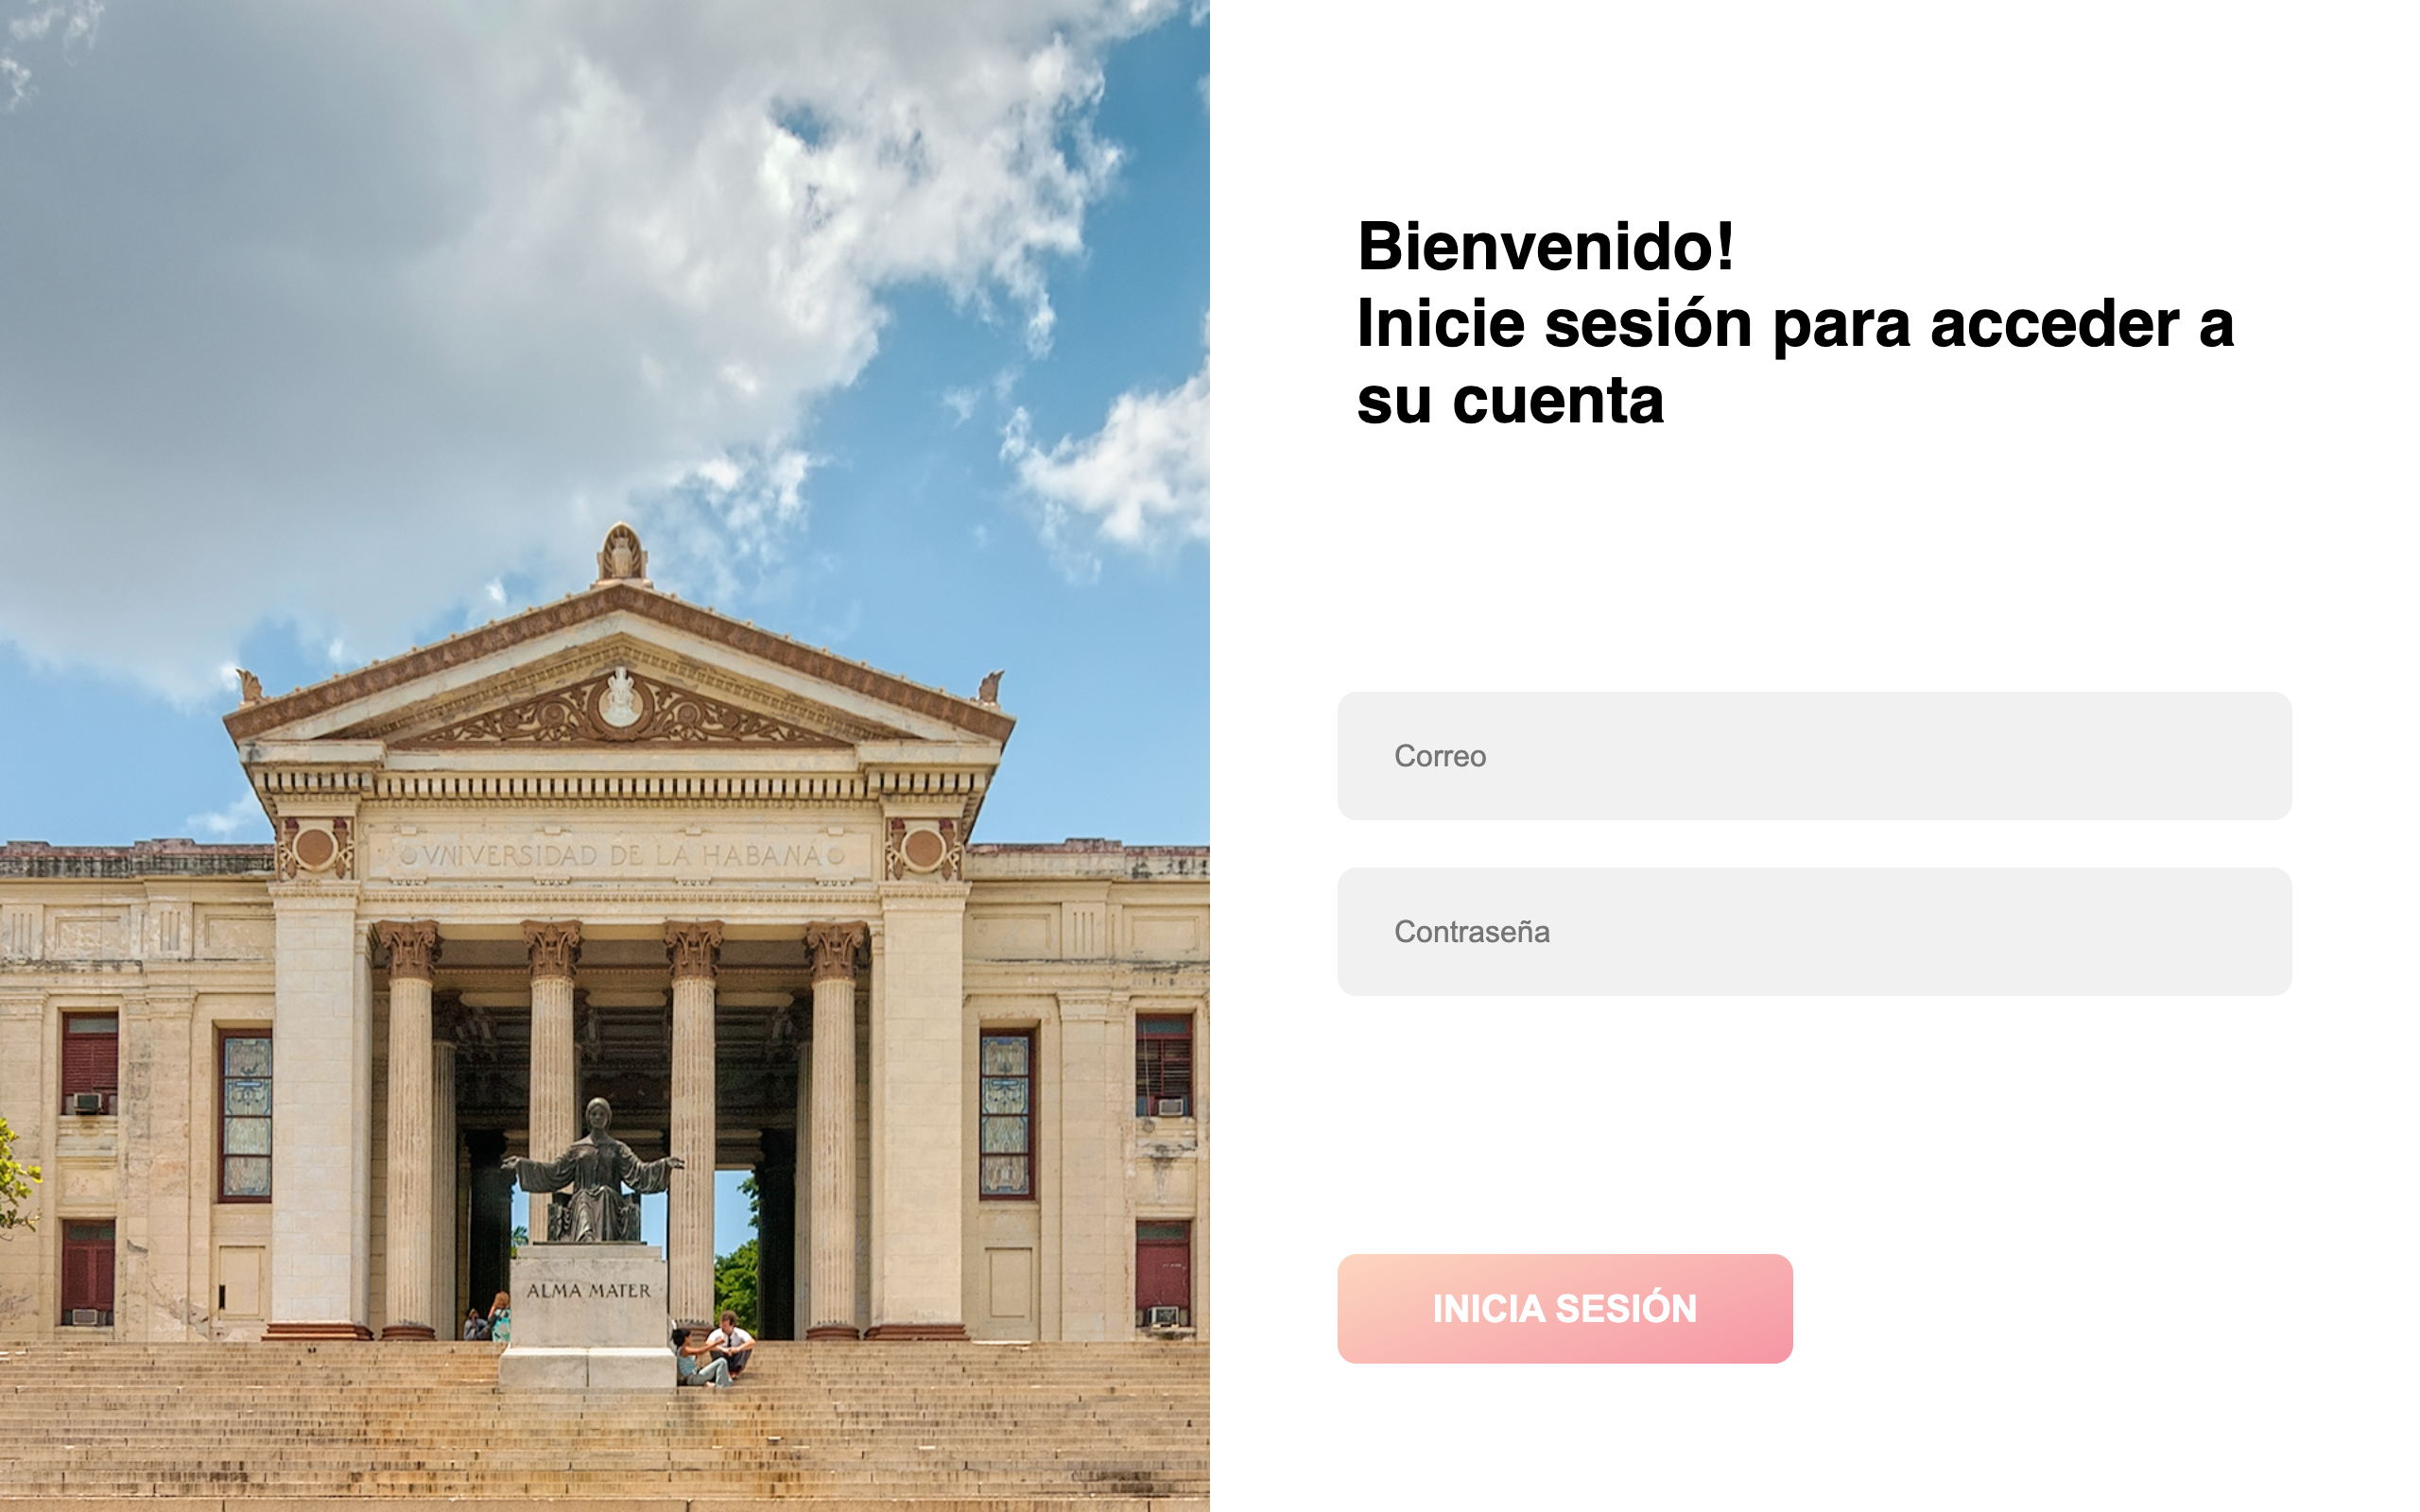
\includegraphics[width=1\linewidth]{Graphics/interfaz}
	\caption{Interfaz visual}
	\label{fig:interfaz}
\end{figure}

Luego de introducir un correo y su correspondiente contraseña se obtiene el token de autenticación y el \textit{refresh token}:

\begin{figure}[H]
	\centering
	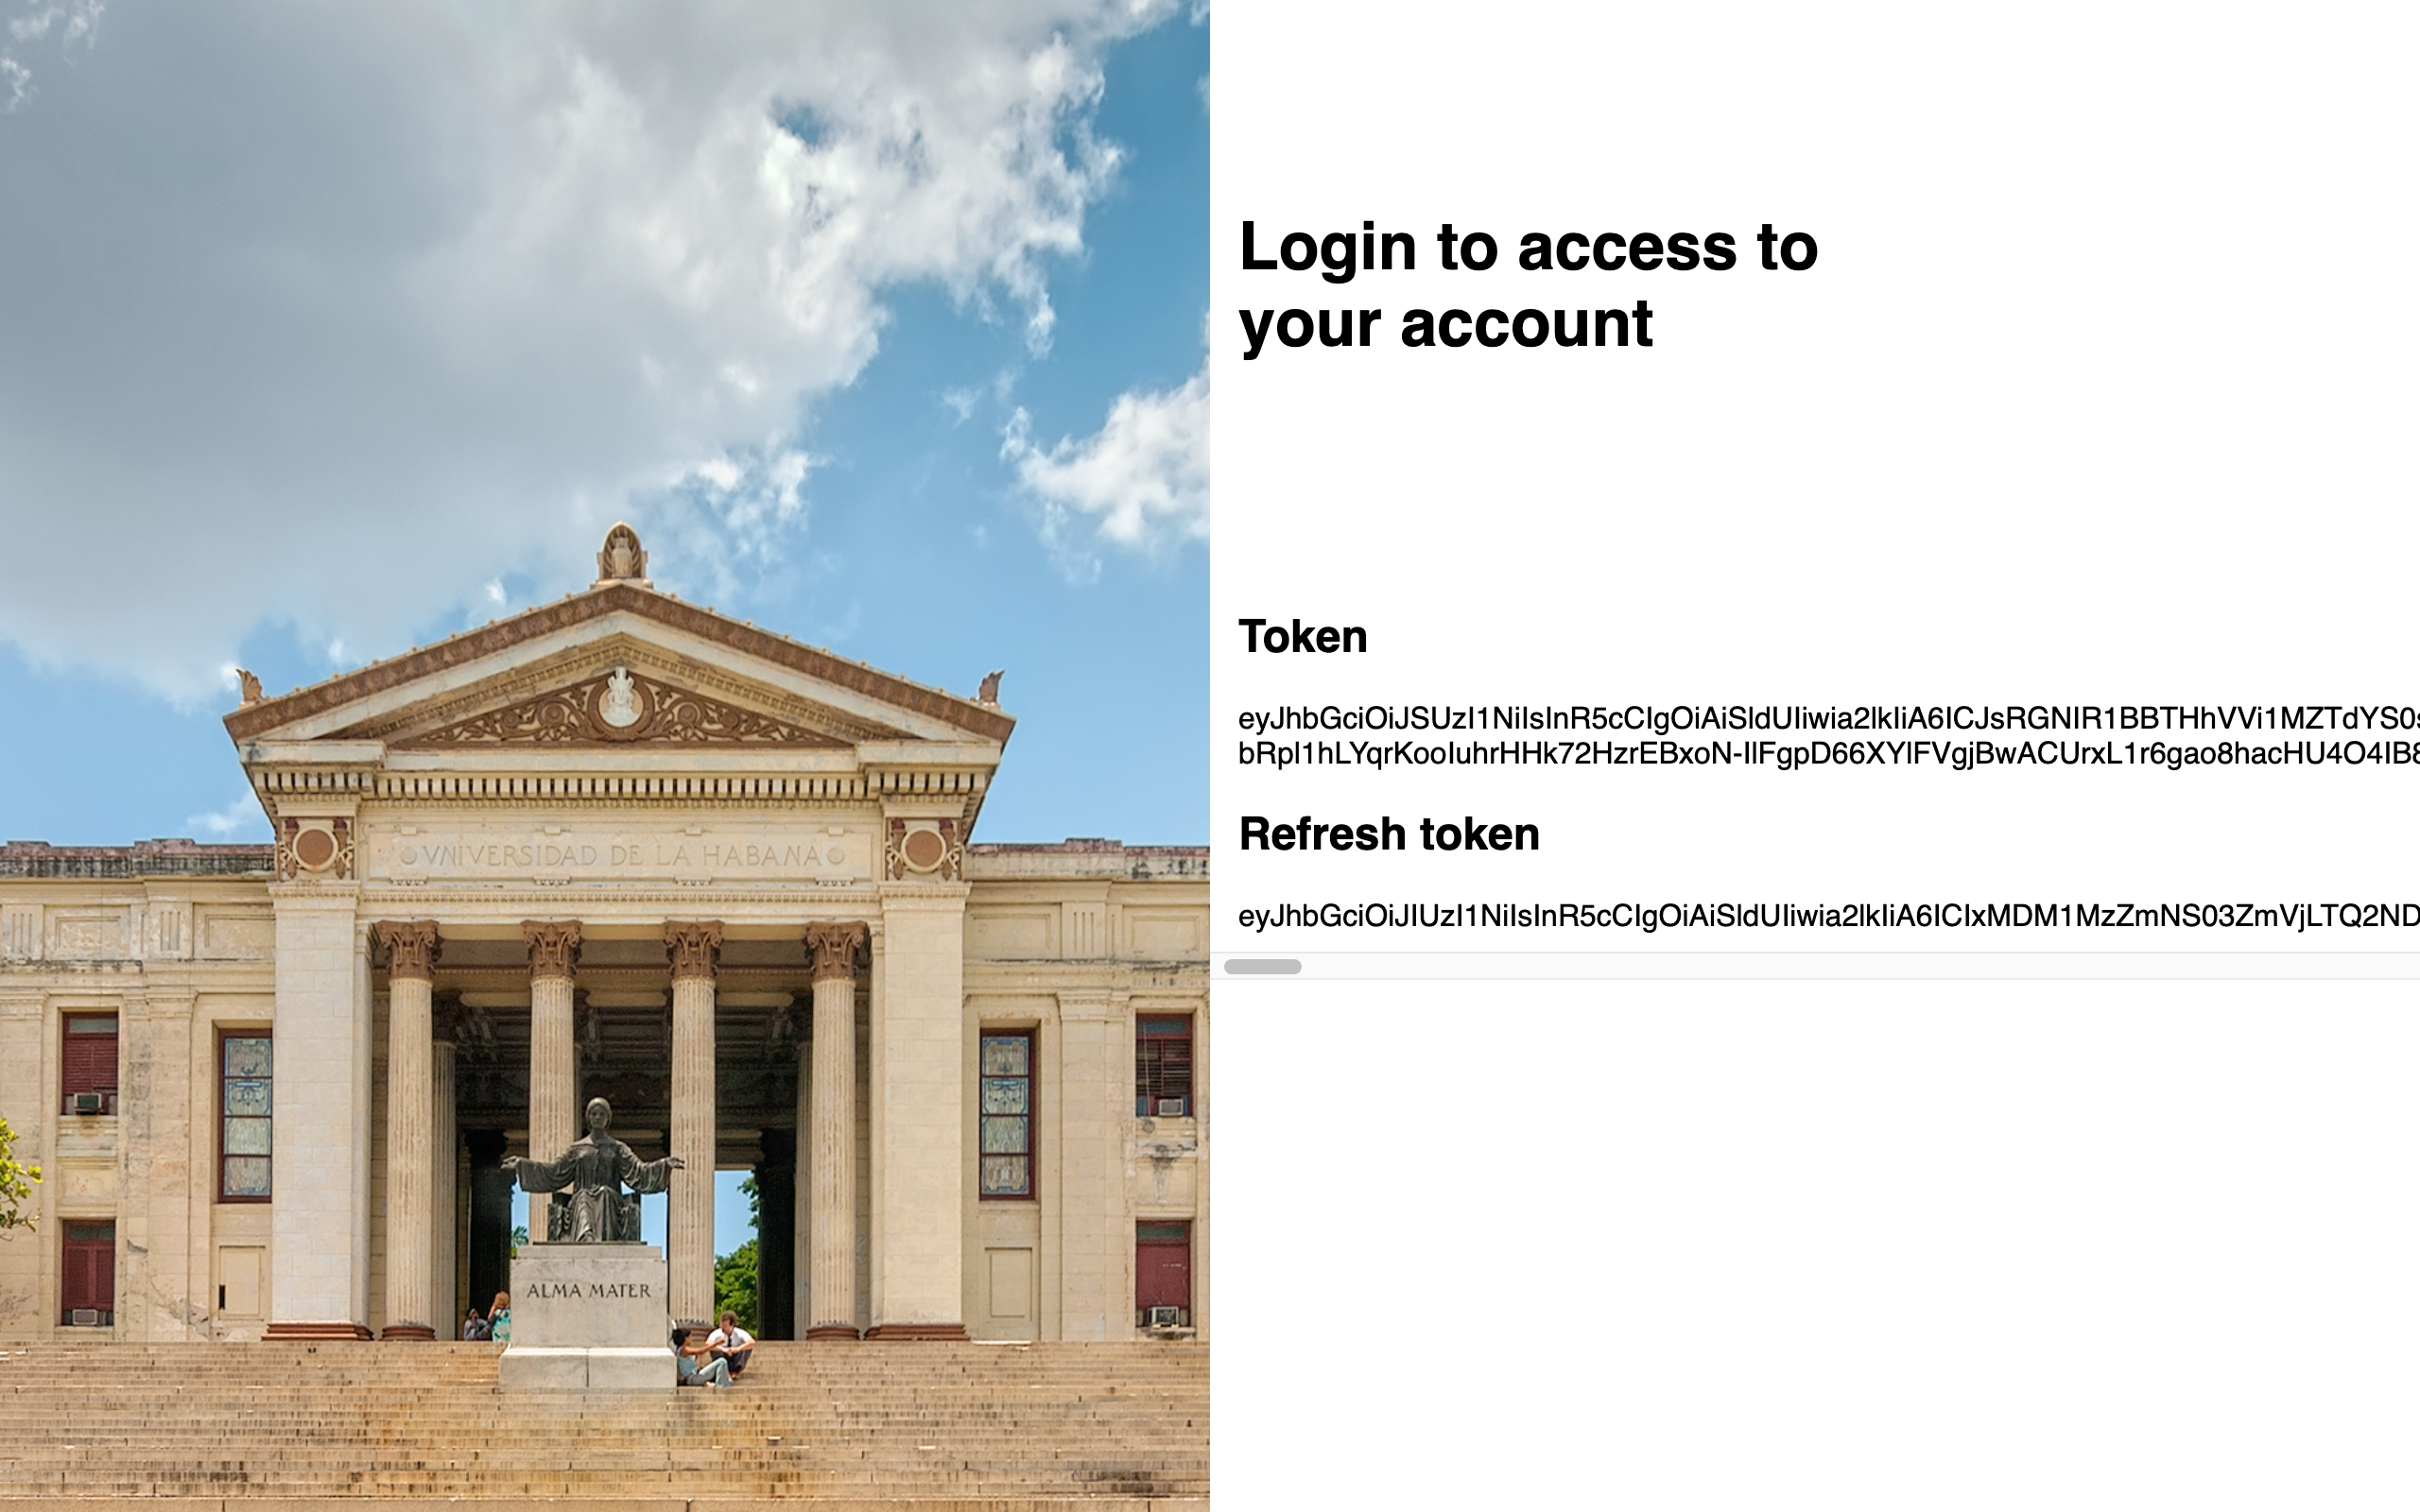
\includegraphics[width=1\linewidth]{Graphics/interfaz_token_success}
	\caption{Resultado de autenticación exitosa}
	\label{fig:interfaztokensuccess}
\end{figure}